\documentclass{article}
\usepackage{makeidx}
\usepackage{hyperref}
\usepackage{amsmath}
\usepackage{amssymb}
\usepackage{xcolor}
\usepackage{graphicx}
\usepackage[top=1in, bottom=1in, left=1in, right=1in]{geometry}

\title{Math Notes}
\author{chtunsw@gmail.com}
\date{}

\makeatletter
\renewcommand\paragraph{\@startsection{paragraph}{4}{\z@}%
                                     {-3.25ex\@plus -1ex \@minus -.2ex}%
                                     {1.5ex \@plus .2ex}%
                                     {\normalfont\normalsize\bfseries}}
\makeatletter

\hypersetup{
    colorlinks=true,
    linkcolor=blue,
    urlcolor=cyan,
}

\setcounter{tocdepth}{4}
\setcounter{secnumdepth}{4}

\makeindex



\begin{document}

\maketitle

\clearpage

\tableofcontents{}

\clearpage

\section{Statistics}

\subsection{Probability Space}

\noindent In probability theory, a probability space or a probability triple \((\Omega, \mathcal{F}, P)\) is a mathematical construct that provides a formal model of a random process or "experiment".

\bigskip

\noindent \(\Omega\): A sample space, which is the set of all possible outcomes of a random process under consideration.

\noindent \(\mathcal{F}\): An event space, which is a set of events, where an event is a subset of outcomes in the sample space. The \(\sigma\)-algebra 
\(\mathcal{F}\) is a collection of all the events we would like to consider.

\noindent \(P\): A probability function, which assigns, to each event in the event space, a probability, which is a number between 0 and 1 (inclusive).

\bigskip

\noindent In the example of the throw of a standard die:

\bigskip

\noindent The sample space  \(\Omega\) is typically the set \(\{1, 2, 3, 4, 5, 6\}\). 

\noindent The event space \(\mathcal{F}\) could be the set of all subsets of the sample space, 
which would then contain simple events such as \(\{5\}\) ("the die lands on 5"),
as well as complex events such as \(\{2, 4, 6\}\) ("the die lands on an even number"). 
So \(\mathcal{F} = \{\{5\}, \{2, 4, 6\}, \dots\}\)

\noindent The probability function \(P\) would then map each event to the number of outcomes in that event divided by 6. 
So for example: \(P(\{5\}) = \frac{1}{6}\), \(P(\{2, 4, 6\}) = \frac{3}{6}\), ...

\subsection{Discrete Probability Distribution}

\noindent Let \(X\) be a random variable with a finite number of finite outcomes \( x_{1},  x_{2}, \ldots, x_{n}\) occurring with probabilities \(p_{1}, p_{2}, \ldots, p_{n}\) respectively. The expectation of \(X\) is defined as

\[\mu = E[X] = \sum_{i=1}^{n}x_{i} p_{i} = x_{1} p_{1} + x_{2} p_{2} + \cdots  + x_{n} p_{n}\]

\noindent The variance of \(X\) is

\[\sigma^{2} = Var(X) = \sum_{i=1}^{n}p_{i} \cdot (x_{i} - \mu)^{2}\]

\noindent For a collection of \(n\) equally likely values:

\[\mu = \frac {1}{n} \sum_{i=1}^{n} x_{i}\]
\[\sigma^{2} = \frac {1}{n} \sum_{i=1}^{n} (x_{i} - \mu)^{2}\]

\noindent \textbf{Expectation}:

\noindent If \(X\) is independent of \(\mathcal{H}\), then \(E(X \mid \mathcal{H}) = E(X)\).

\noindent Tower property: for sub-\(\sigma\)-algebras \(\mathcal{H}_1 \subseteq \mathcal{H}_2 \subseteq \mathcal{F}\), then \(E(E(X \mid \mathcal{H}_2) \mid \mathcal{H}_1) = E(X \mid \mathcal{H}_1)\).

\noindent Law of total expectation: \(E(E(X \mid \mathcal{H})) = E(X)\). A special case of tower property when \(\mathcal{H}_1 = \{\emptyset, \Omega\}\).

\noindent Linearity:
\(E(X_{1}+X_{2}\mid {\mathcal {H}})=E(X_{1}\mid {\mathcal {H}})+E(X_{2}\mid {\mathcal {H}})\) and, 
\(E(aX \mid {\mathcal {H}}) = a E(X \mid {\mathcal {H}})\) when \(a \in \mathbb {R}\).

\subsection{Continuous Probability Distribution}

\noindent If the random variable \(X\) has a probability density function \(f(x)\), and \(F(x)\) is the corresponding cumulative distribution function, then

\[P(a \leq X \leq b) = \int_{a}^{b} f(x)dx\]
\[F(x) = P(X \leq x) = \int_{-\infty}^{x} f(t)dt\]
\[\mu =\int_{\mathbb{R}} x f(x) dx = \int_{\mathbb{R}} x dF(x)\]
\[\sigma^{2} = \int_{\mathbb{R}}(x - \mu)^{2} f(x) dx\]

\subsubsection{Uniform Distribution}

\begin{center}
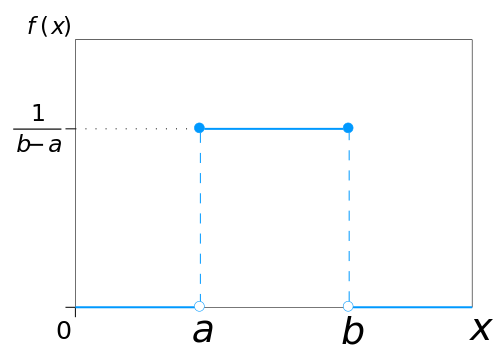
\includegraphics[scale=0.4]{./images/uniform_distribution.png}
\end{center}

\[
f(x) = 
\begin{cases}
\frac{1}{b-a} & \mathrm{for} \ a \leq x \leq b, \\
0 & \mathrm{for} \ x < a \ \mathrm{or} \ x > b
\end{cases}
\]
\[\mu = \tfrac{1}{2} (a + b)\]
\[\sigma^{2} = \tfrac{1}{12} (b - a)^{2}\]

\subsubsection{Normal Distribution}

\begin{center}
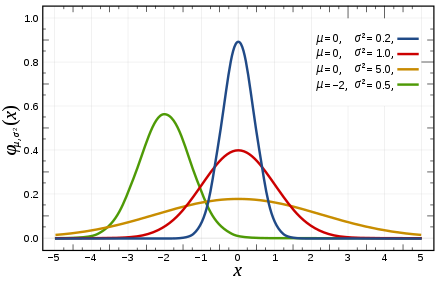
\includegraphics[scale=0.4]{./images/normal_distribution.png}
\end{center}

\[f(x) = \frac{1}{\sigma \sqrt{2\pi}} e^{-\frac{1}{2} (\frac{x - \mu}{\sigma })^{2}}\]

\section{Mathematical Analysis}

\subsection{Metric Space}

\noindent A metric space is an ordered pair \((M, d)\) where \(M\) is a set and \(d\) is a distance metric (function) on \(M\),

\[d: M \times M \rightarrow \mathbb{R}\]

\noindent satisfying the following axioms for all points \(x, y, z \in M\):

\begin{itemize}
    \item The distance from a point to itself is zero: \(d(x, x) = 0\)
    \item (Positivity) The distance between two distinct points is always positive: If \(x \neq y\), then \(d(x,y) > 0\)
    \item (Symmetry) The distance from \(x\) to \(y\) is always the same as the distance from \(y\) to \(x\): \(d(x,y) = d(y,x)\)
    \item The triangle inequality holds: \(d(x, z) \leq  d(x, y) + d(y, z)\)
\end{itemize}

\subsubsection{Contraction Mapping}

\noindent In mathematics, a contraction mapping, or contraction or contractor, on a metric space \((M, d)\) is a function \(f\) from \(M\) to itself, 
aka contraction mapping \(f: M \rightarrow M\), with the property that there is some real number \(0 \leq k < 1\) such that for all \(x\) and \(y\) in \(M\),

\[d(f(x), f(y)) \leq k d(x, y)\]

\printindex

\end{document}